\documentclass[twoside]{book}

% Packages required by doxygen
\usepackage{fixltx2e}
\usepackage{calc}
\usepackage{doxygen}
\usepackage{graphicx}
\usepackage[utf8]{inputenc}
\usepackage{makeidx}
\usepackage{multicol}
\usepackage{multirow}
\PassOptionsToPackage{warn}{textcomp}
\usepackage{textcomp}
\usepackage[nointegrals]{wasysym}
\usepackage[table]{xcolor}

% NLS support packages
\usepackage[french]{babel}

% Font selection
\usepackage[T1]{fontenc}
\usepackage{mathptmx}
\usepackage[scaled=.90]{helvet}
\usepackage{courier}
\usepackage{amssymb}
\usepackage{sectsty}
\renewcommand{\familydefault}{\sfdefault}
\allsectionsfont{%
  \fontseries{bc}\selectfont%
  \color{darkgray}%
}
\renewcommand{\DoxyLabelFont}{%
  \fontseries{bc}\selectfont%
  \color{darkgray}%
}
\newcommand{\+}{\discretionary{\mbox{\scriptsize$\hookleftarrow$}}{}{}}

% Page & text layout
\usepackage{geometry}
\geometry{%
  a4paper,%
  top=2.5cm,%
  bottom=2.5cm,%
  left=2.5cm,%
  right=2.5cm%
}
\tolerance=750
\hfuzz=15pt
\hbadness=750
\setlength{\emergencystretch}{15pt}
\setlength{\parindent}{0cm}
\setlength{\parskip}{0.2cm}
\makeatletter
\renewcommand{\paragraph}{%
  \@startsection{paragraph}{4}{0ex}{-1.0ex}{1.0ex}{%
    \normalfont\normalsize\bfseries\SS@parafont%
  }%
}
\renewcommand{\subparagraph}{%
  \@startsection{subparagraph}{5}{0ex}{-1.0ex}{1.0ex}{%
    \normalfont\normalsize\bfseries\SS@subparafont%
  }%
}
\makeatother

% Headers & footers
\usepackage{fancyhdr}
\pagestyle{fancyplain}
\fancyhead[LE]{\fancyplain{}{\bfseries\thepage}}
\fancyhead[CE]{\fancyplain{}{}}
\fancyhead[RE]{\fancyplain{}{\bfseries\leftmark}}
\fancyhead[LO]{\fancyplain{}{\bfseries\rightmark}}
\fancyhead[CO]{\fancyplain{}{}}
\fancyhead[RO]{\fancyplain{}{\bfseries\thepage}}
\fancyfoot[LE]{\fancyplain{}{}}
\fancyfoot[CE]{\fancyplain{}{}}
\fancyfoot[RE]{\fancyplain{}{\bfseries\scriptsize Généré le Mardi 13 Janvier 2015 01\+:23\+:07 pour Projet informatique par Doxygen }}
\fancyfoot[LO]{\fancyplain{}{\bfseries\scriptsize Généré le Mardi 13 Janvier 2015 01\+:23\+:07 pour Projet informatique par Doxygen }}
\fancyfoot[CO]{\fancyplain{}{}}
\fancyfoot[RO]{\fancyplain{}{}}
\renewcommand{\footrulewidth}{0.4pt}
\renewcommand{\chaptermark}[1]{%
  \markboth{#1}{}%
}
\renewcommand{\sectionmark}[1]{%
  \markright{\thesection\ #1}%
}

% Indices & bibliography
\usepackage{natbib}
\usepackage[titles]{tocloft}
\setcounter{tocdepth}{3}
\setcounter{secnumdepth}{5}
\makeindex

% Hyperlinks (required, but should be loaded last)
\usepackage{ifpdf}
\ifpdf
  \usepackage[pdftex,pagebackref=true]{hyperref}
\else
  \usepackage[ps2pdf,pagebackref=true]{hyperref}
\fi
\hypersetup{%
  colorlinks=true,%
  linkcolor=blue,%
  citecolor=blue,%
  unicode%
}

% Custom commands
\newcommand{\clearemptydoublepage}{%
  \newpage{\pagestyle{empty}\cleardoublepage}%
}


%===== C O N T E N T S =====

\begin{document}

% Titlepage & ToC
\hypersetup{pageanchor=false,
             bookmarks=true,
             bookmarksnumbered=true,
             pdfencoding=unicode
            }
\pagenumbering{roman}
\begin{titlepage}
\vspace*{7cm}
\begin{center}%
{\Large Projet informatique }\\
\vspace*{1cm}
{\large Généré par Doxygen 1.8.8}\\
\vspace*{0.5cm}
{\small Mardi 13 Janvier 2015 01:23:07}\\
\end{center}
\end{titlepage}
\clearemptydoublepage
\tableofcontents
\clearemptydoublepage
\pagenumbering{arabic}
\hypersetup{pageanchor=true}

%--- Begin generated contents ---
\chapter{Index des classes}
\section{Liste des classes}
Liste des classes, structures, unions et interfaces avec une brève description \+:\begin{DoxyCompactList}
\item\contentsline{section}{\hyperlink{structt__fourmi}{t\+\_\+fourmi} \\*Structure necessaire a la connaissance de Zozor, avec sa place en x, y et son numero d'immatriculation }{\pageref{structt__fourmi}}{}
\end{DoxyCompactList}

\chapter{Index des fichiers}
\section{Liste des fichiers}
Liste de tous les fichiers documentés avec une brève description \+:\begin{DoxyCompactList}
\item\contentsline{section}{\hyperlink{affichage_8c}{affichage.\+c} \\*Definition des fonctions d'affichage }{\pageref{affichage_8c}}{}
\item\contentsline{section}{\hyperlink{aleatoire_8c}{aleatoire.\+c} \\*Page permettant de creer de l'aleatoire }{\pageref{aleatoire_8c}}{}
\item\contentsline{section}{\hyperlink{deplacement_8c}{deplacement.\+c} \\*Page contenant le deplacement de Zozor }{\pageref{deplacement_8c}}{}
\item\contentsline{section}{\hyperlink{fin__de__jeu_8c}{fin\+\_\+de\+\_\+jeu.\+c} \\*Page contenant la fin de jeu }{\pageref{fin__de__jeu_8c}}{}
\item\contentsline{section}{\hyperlink{fourmi_8c}{fourmi.\+c} \\*Page contenant les fonctions relatives a la de la fourmi et de tout ce qui y touche }{\pageref{fourmi_8c}}{}
\item\contentsline{section}{\hyperlink{gen__fourmi_8c}{gen\+\_\+fourmi.\+c} \\*Page contenant les fonctions relatives a la de Zozor et de tout ce qui y touche }{\pageref{gen__fourmi_8c}}{}
\item\contentsline{section}{\hyperlink{gen__labyrinthe_8c}{gen\+\_\+labyrinthe.\+c} \\*Page contenant les fonctions relatives a la creation du labyrinthe, et la mise en place des points strategiques }{\pageref{gen__labyrinthe_8c}}{}
\item\contentsline{section}{\hyperlink{header_8h}{header.\+h} \\*Header contenant les definition des fonctions necessaire au \hyperlink{main_8c}{main.\+c} }{\pageref{header_8h}}{}
\item\contentsline{section}{\hyperlink{header__fourmi_8h}{header\+\_\+fourmi.\+h} \\*Header contenant les definition des fonctions necessaire au fonction de génération des fourmis et de leurs déplacements }{\pageref{header__fourmi_8h}}{}
\item\contentsline{section}{\hyperlink{main_8c}{main.\+c} \\*Simulation de la vie d'un groupe de Zozor dans un labyrinthe }{\pageref{main_8c}}{}
\item\contentsline{section}{\hyperlink{mise__a__0_8c}{mise\+\_\+a\+\_\+0.\+c} \\*D�finition des fonctions de mise a zero d'une matrice, ou de mise a l'�tat vide }{\pageref{mise__a__0_8c}}{}
\item\contentsline{section}{\hyperlink{stock_8c}{stock.\+c} \\*D�finition des fonctions permettant de gerer les stocks de chaques points, de la cr�ation au retrait }{\pageref{stock_8c}}{}
\item\contentsline{section}{\hyperlink{verification__saisie_8c}{verification\+\_\+saisie.\+c} \\*Page permettant de v�rifier la saisie de l'utilisateur }{\pageref{verification__saisie_8c}}{}
\end{DoxyCompactList}

\chapter{Documentation des classes}
\hypertarget{structt__fourmi}{\section{Référence de la structure t\+\_\+fourmi}
\label{structt__fourmi}\index{t\+\_\+fourmi@{t\+\_\+fourmi}}
}
\subsection*{Attributs publics}
\begin{DoxyCompactItemize}
\item 
\hypertarget{structt__fourmi_ab45e723a7a11d7789888a5ee574c6bc9}{int {\bfseries matricule}}\label{structt__fourmi_ab45e723a7a11d7789888a5ee574c6bc9}

\item 
\hypertarget{structt__fourmi_a258cf4f2243aad27ab01dc55bb701078}{int {\bfseries x}}\label{structt__fourmi_a258cf4f2243aad27ab01dc55bb701078}

\item 
\hypertarget{structt__fourmi_aa9fe73b8d3d492ce6cf3985e4910fdf2}{int {\bfseries y}}\label{structt__fourmi_aa9fe73b8d3d492ce6cf3985e4910fdf2}

\item 
\hypertarget{structt__fourmi_a757c3ee4ea2dcbf825cd93f6b8bf0ef8}{int {\bfseries eau}}\label{structt__fourmi_a757c3ee4ea2dcbf825cd93f6b8bf0ef8}

\item 
\hypertarget{structt__fourmi_a0a2a75c5a649f263d4e299a488edfe4f}{int {\bfseries dodo}}\label{structt__fourmi_a0a2a75c5a649f263d4e299a488edfe4f}

\item 
\hypertarget{structt__fourmi_a5ba7caca7f8cf1e8195ceae92cdaca00}{int {\bfseries repas}}\label{structt__fourmi_a5ba7caca7f8cf1e8195ceae92cdaca00}

\item 
\hypertarget{structt__fourmi_a81345593813fffd4760b20bc55392190}{int {\bfseries total\+\_\+mv}}\label{structt__fourmi_a81345593813fffd4760b20bc55392190}

\end{DoxyCompactItemize}


La documentation de cette structure a été générée à partir du fichier suivant \+:\begin{DoxyCompactItemize}
\item 
header.\+h\end{DoxyCompactItemize}

\chapter{Documentation des fichiers}
\hypertarget{affichage_8c}{\section{Référence du fichier affichage.\+c}
\label{affichage_8c}\index{affichage.\+c@{affichage.\+c}}
}


Definition des fonctions d'affichage.  


{\ttfamily \#include \char`\"{}header.\+h\char`\"{}}\\*
Graphe des dépendances par inclusion de affichage.\+c\+:\nopagebreak
\begin{figure}[H]
\begin{center}
\leavevmode
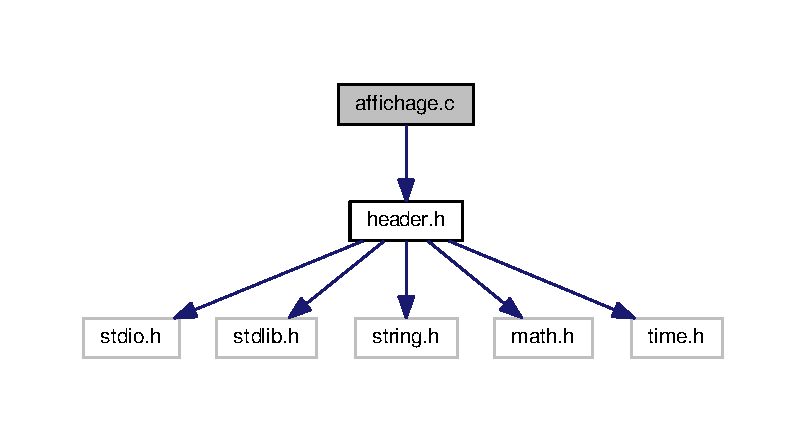
\includegraphics[width=350pt]{affichage_8c__incl}
\end{center}
\end{figure}
\subsection*{Fonctions}
\begin{DoxyCompactItemize}
\item 
\hypertarget{affichage_8c_a42ec04270a0e1a044bcbec3d08bc9f0a}{void \hyperlink{affichage_8c_a42ec04270a0e1a044bcbec3d08bc9f0a}{affiche\+\_\+lab} (void)}\label{affichage_8c_a42ec04270a0e1a044bcbec3d08bc9f0a}

\begin{DoxyCompactList}\small\item\em Fonction d'affichage du labyrinthe. \end{DoxyCompactList}\item 
void \hyperlink{affichage_8c_afdabedbdaec06f1a4ab234044b4df6fc}{affiche\+\_\+entrer} (int tmp)
\begin{DoxyCompactList}\small\item\em Fonction permettant l'affichage d'un certain nombre de ligne vide. \end{DoxyCompactList}\end{DoxyCompactItemize}


\subsection{Description détaillée}
Definition des fonctions d'affichage. 

\begin{DoxyAuthor}{Auteur}
Jean-\/baptiste Dubois, Provost Valentin, Dezere Florian 
\end{DoxyAuthor}
\begin{DoxyVersion}{Version}
1.\+0 
\end{DoxyVersion}
\begin{DoxyDate}{Date}
6 Janvier 2014 
\end{DoxyDate}


\subsection{Documentation des fonctions}
\hypertarget{affichage_8c_afdabedbdaec06f1a4ab234044b4df6fc}{\index{affichage.\+c@{affichage.\+c}!affiche\+\_\+entrer@{affiche\+\_\+entrer}}
\index{affiche\+\_\+entrer@{affiche\+\_\+entrer}!affichage.\+c@{affichage.\+c}}
\subsubsection[{affiche\+\_\+entrer}]{\setlength{\rightskip}{0pt plus 5cm}void affiche\+\_\+entrer (
\begin{DoxyParamCaption}
\item[{int}]{tmp}
\end{DoxyParamCaption}
)}}\label{affichage_8c_afdabedbdaec06f1a4ab234044b4df6fc}


Fonction permettant l'affichage d'un certain nombre de ligne vide. 


\begin{DoxyParams}{Paramètres}
{\em int} & tmp nombre de retour chariot � afficher \\
\hline
\end{DoxyParams}

\hypertarget{aleatoire_8c}{\section{Référence du fichier aleatoire.\+c}
\label{aleatoire_8c}\index{aleatoire.\+c@{aleatoire.\+c}}
}


Page permettant de creer de l'aleatoire.  


{\ttfamily \#include \char`\"{}header.\+h\char`\"{}}\\*
Graphe des dépendances par inclusion de aleatoire.\+c\+:
\nopagebreak
\begin{figure}[H]
\begin{center}
\leavevmode
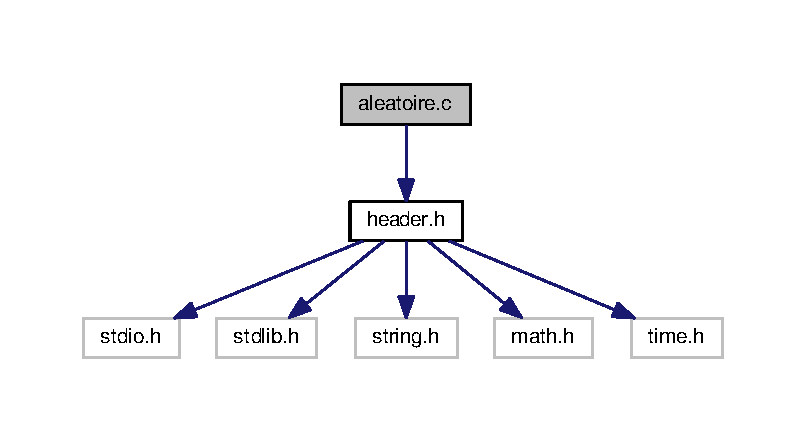
\includegraphics[width=350pt]{aleatoire_8c__incl}
\end{center}
\end{figure}
\subsection*{Fonctions}
\begin{DoxyCompactItemize}
\item 
\hypertarget{aleatoire_8c_aaeeedbd134251291fe79c71c943ec899}{void \hyperlink{aleatoire_8c_aaeeedbd134251291fe79c71c943ec899}{aleatoire} (void)}\label{aleatoire_8c_aaeeedbd134251291fe79c71c943ec899}

\begin{DoxyCompactList}\small\item\em Fonction permettant de creer l'aleatoire. \end{DoxyCompactList}\end{DoxyCompactItemize}


\subsection{Description détaillée}
Page permettant de creer de l'aleatoire. 

\begin{DoxyAuthor}{Auteur}
Jean-\/baptiste Dubois, Provost Valentin, Dezere Florian 
\end{DoxyAuthor}
\begin{DoxyVersion}{Version}
1.\+0 
\end{DoxyVersion}
\begin{DoxyDate}{Date}
6 Janvier 2014 
\end{DoxyDate}

\hypertarget{deplacement_8c}{\section{Référence du fichier deplacement.\+c}
\label{deplacement_8c}\index{deplacement.\+c@{deplacement.\+c}}
}


Page contenant le deplacement de Zozor.  


{\ttfamily \#include \char`\"{}header.\+h\char`\"{}}\\*
Graphe des dépendances par inclusion de deplacement.\+c\+:\nopagebreak
\begin{figure}[H]
\begin{center}
\leavevmode
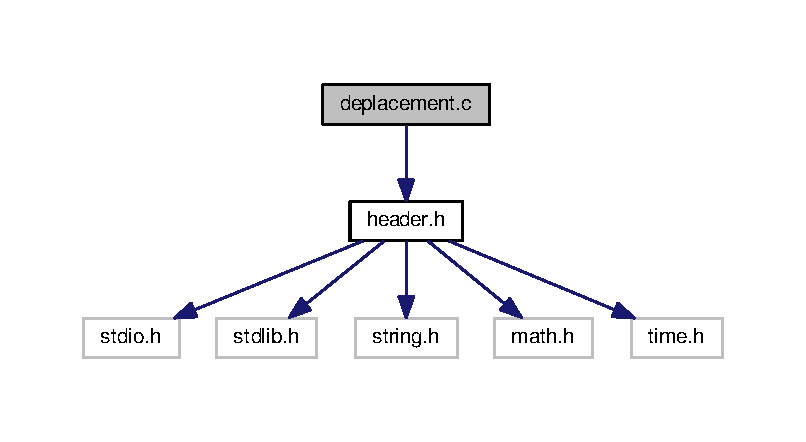
\includegraphics[width=350pt]{deplacement_8c__incl}
\end{center}
\end{figure}
\subsection*{Fonctions}
\begin{DoxyCompactItemize}
\item 
int \hyperlink{deplacement_8c_a022b37db62e51a6efc03eee80cda50cd}{verif\+\_\+deplacement} (int id\+\_\+fourmi)
\begin{DoxyCompactList}\small\item\em Fonction permettant de verifier si Zozor peut se deplacer. \end{DoxyCompactList}\item 
void \hyperlink{deplacement_8c_a851f3d658198e4622f03e2d8a7faec14}{mv\+\_\+fourmi} (int id\+\_\+fourmi)
\begin{DoxyCompactList}\small\item\em Fonction permettant le deplacement des fourmis dans le labyrinthe de fa�on aleatoire. \end{DoxyCompactList}\end{DoxyCompactItemize}


\subsection{Description détaillée}
Page contenant le deplacement de Zozor. 

\begin{DoxyAuthor}{Auteur}
Jean-\/baptiste Dubois, Provost Valentin, Dezere Florian 
\end{DoxyAuthor}
\begin{DoxyVersion}{Version}
1.\+0 
\end{DoxyVersion}
\begin{DoxyDate}{Date}
6 Janvier 2014 
\end{DoxyDate}


\subsection{Documentation des fonctions}
\hypertarget{deplacement_8c_a851f3d658198e4622f03e2d8a7faec14}{\index{deplacement.\+c@{deplacement.\+c}!mv\+\_\+fourmi@{mv\+\_\+fourmi}}
\index{mv\+\_\+fourmi@{mv\+\_\+fourmi}!deplacement.\+c@{deplacement.\+c}}
\subsubsection[{mv\+\_\+fourmi}]{\setlength{\rightskip}{0pt plus 5cm}void mv\+\_\+fourmi (
\begin{DoxyParamCaption}
\item[{int}]{id\+\_\+fourmi}
\end{DoxyParamCaption}
)}}\label{deplacement_8c_a851f3d658198e4622f03e2d8a7faec14}


Fonction permettant le deplacement des fourmis dans le labyrinthe de fa�on aleatoire. 


\begin{DoxyParams}{Paramètres}
{\em int} & id\+\_\+fourmi est l'identifiant de Zozor \\
\hline
\end{DoxyParams}
\hypertarget{deplacement_8c_a022b37db62e51a6efc03eee80cda50cd}{\index{deplacement.\+c@{deplacement.\+c}!verif\+\_\+deplacement@{verif\+\_\+deplacement}}
\index{verif\+\_\+deplacement@{verif\+\_\+deplacement}!deplacement.\+c@{deplacement.\+c}}
\subsubsection[{verif\+\_\+deplacement}]{\setlength{\rightskip}{0pt plus 5cm}int verif\+\_\+deplacement (
\begin{DoxyParamCaption}
\item[{int}]{id\+\_\+fourmi}
\end{DoxyParamCaption}
)}}\label{deplacement_8c_a022b37db62e51a6efc03eee80cda50cd}


Fonction permettant de verifier si Zozor peut se deplacer. 


\begin{DoxyParams}{Paramètres}
{\em int} & id\+\_\+fourmi est l'identifiant de Zozor \\
\hline
\end{DoxyParams}
\begin{DoxyReturn}{Renvoie}
renvoi vrai si le d�placement peut avoir lieu sinon faux 
\end{DoxyReturn}

\hypertarget{fin__de__jeu_8c}{\section{Référence du fichier fin\+\_\+de\+\_\+jeu.\+c}
\label{fin__de__jeu_8c}\index{fin\+\_\+de\+\_\+jeu.\+c@{fin\+\_\+de\+\_\+jeu.\+c}}
}


Page contenant la fin de jeu.  


{\ttfamily \#include \char`\"{}header.\+h\char`\"{}}\\*
Graphe des dépendances par inclusion de fin\+\_\+de\+\_\+jeu.\+c\+:
\nopagebreak
\begin{figure}[H]
\begin{center}
\leavevmode
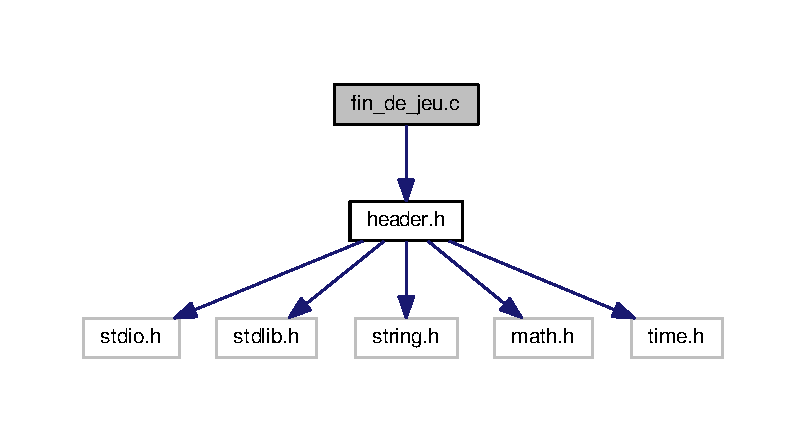
\includegraphics[width=350pt]{fin__de__jeu_8c__incl}
\end{center}
\end{figure}
\subsection*{Fonctions}
\begin{DoxyCompactItemize}
\item 
\hypertarget{fin__de__jeu_8c_a5b977cd2b36e961cb4b9382e91ade34b}{int \hyperlink{fin__de__jeu_8c_a5b977cd2b36e961cb4b9382e91ade34b}{end\+\_\+game} (void)}\label{fin__de__jeu_8c_a5b977cd2b36e961cb4b9382e91ade34b}

\begin{DoxyCompactList}\small\item\em Fonction permettant de savoir si la troll case met fin a la partie. \end{DoxyCompactList}\item 
\hypertarget{fin__de__jeu_8c_ad9fd7e15b3676ff1d6f05821968adf54}{void \hyperlink{fin__de__jeu_8c_ad9fd7e15b3676ff1d6f05821968adf54}{gen\+\_\+troll\+\_\+case} (void)}\label{fin__de__jeu_8c_ad9fd7e15b3676ff1d6f05821968adf54}

\begin{DoxyCompactList}\small\item\em Fonction permettant la generation de la troll case, qui peut mettre fin a la partie. \end{DoxyCompactList}\end{DoxyCompactItemize}


\subsection{Description détaillée}
Page contenant la fin de jeu. 

\begin{DoxyAuthor}{Auteur}
Jean-\/baptiste Dubois, Provost Valentin, Dezere Florian 
\end{DoxyAuthor}
\begin{DoxyVersion}{Version}
1.\+0 
\end{DoxyVersion}
\begin{DoxyDate}{Date}
6 Janvier 2014 
\end{DoxyDate}

\hypertarget{fourmi_8c}{\section{Référence du fichier fourmi.\+c}
\label{fourmi_8c}\index{fourmi.\+c@{fourmi.\+c}}
}


Page contenant les fonctions relatives a la de la fourmi et de tout ce qui y touche.  


{\ttfamily \#include \char`\"{}header.\+h\char`\"{}}\\*
{\ttfamily \#include \char`\"{}header\+\_\+fourmi.\+h\char`\"{}}\\*
Graphe des dépendances par inclusion de fourmi.\+c\+:
\nopagebreak
\begin{figure}[H]
\begin{center}
\leavevmode
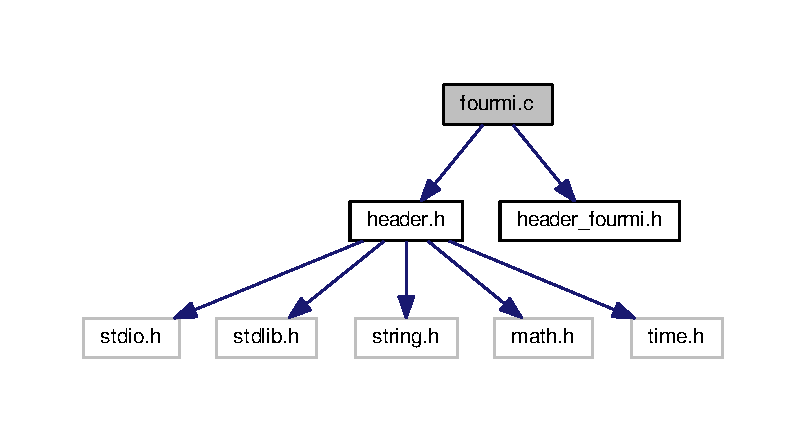
\includegraphics[width=350pt]{fourmi_8c__incl}
\end{center}
\end{figure}
\subsection*{Fonctions}
\begin{DoxyCompactItemize}
\item 
void \hyperlink{fourmi_8c_ae621d3f12ff30448e45c4e134d049b03}{gen\+\_\+fourmi} (void)
\begin{DoxyCompactList}\small\item\em Fonction permettant le pop des fourmis. \end{DoxyCompactList}\item 
void \hyperlink{fourmi_8c_ae0cc7c685736b97de5cd92845f3730d3}{gen\+\_\+stock\+\_\+fourmi} (int id\+\_\+fourmi)
\begin{DoxyCompactList}\small\item\em Fonction permettant de definir une quantite de nourriture, d'eau, de dodo que possede Zozor. \end{DoxyCompactList}\item 
void \hyperlink{fourmi_8c_add23d0755a1059dab2f4e326d1c8f2c5}{etat\+\_\+fourmi} (int id\+\_\+fourmi)
\begin{DoxyCompactList}\small\item\em Fonction permettant d'afficher l'etat de Zozor, sa quantite de repas, d'eau et de sommeil disponible. \end{DoxyCompactList}\item 
void \hyperlink{fourmi_8c_a85661a77431adbf32f45d1b707c270e2}{recherche\+\_\+base} (int $\ast$x, int $\ast$y)
\begin{DoxyCompactList}\small\item\em Fonction permettant la recherche de la base du labyrinthe pour le pop de Zozor. \end{DoxyCompactList}\end{DoxyCompactItemize}


\subsection{Description détaillée}
Page contenant les fonctions relatives a la de la fourmi et de tout ce qui y touche. 

\begin{DoxyAuthor}{Auteur}
Jean-\/baptiste Dubois, Provost Valentin, Dezere Florian 
\end{DoxyAuthor}
\begin{DoxyVersion}{Version}
1.\+0 
\end{DoxyVersion}
\begin{DoxyDate}{Date}
6 Janvier 2014 
\end{DoxyDate}


\subsection{Documentation des fonctions}
\hypertarget{fourmi_8c_add23d0755a1059dab2f4e326d1c8f2c5}{\index{fourmi.\+c@{fourmi.\+c}!etat\+\_\+fourmi@{etat\+\_\+fourmi}}
\index{etat\+\_\+fourmi@{etat\+\_\+fourmi}!fourmi.\+c@{fourmi.\+c}}
\subsubsection[{etat\+\_\+fourmi}]{\setlength{\rightskip}{0pt plus 5cm}void etat\+\_\+fourmi (
\begin{DoxyParamCaption}
\item[{int}]{id\+\_\+fourmi}
\end{DoxyParamCaption}
)}}\label{fourmi_8c_add23d0755a1059dab2f4e326d1c8f2c5}


Fonction permettant d'afficher l'etat de Zozor, sa quantite de repas, d'eau et de sommeil disponible. 

fonction permettant d'afficher l'etat de Zozor, sa quantite de repas, d'eau et de sommeil disponible


\begin{DoxyParams}{Paramètres}
{\em int} & id\+\_\+fourmi est l'identifiant de Zozor \\
\hline
\end{DoxyParams}
\hypertarget{fourmi_8c_ae621d3f12ff30448e45c4e134d049b03}{\index{fourmi.\+c@{fourmi.\+c}!gen\+\_\+fourmi@{gen\+\_\+fourmi}}
\index{gen\+\_\+fourmi@{gen\+\_\+fourmi}!fourmi.\+c@{fourmi.\+c}}
\subsubsection[{gen\+\_\+fourmi}]{\setlength{\rightskip}{0pt plus 5cm}void gen\+\_\+fourmi (
\begin{DoxyParamCaption}
\item[{void}]{}
\end{DoxyParamCaption}
)}}\label{fourmi_8c_ae621d3f12ff30448e45c4e134d049b03}


Fonction permettant le pop des fourmis. 

fonction permettant le pop de Zozor \hypertarget{fourmi_8c_ae0cc7c685736b97de5cd92845f3730d3}{\index{fourmi.\+c@{fourmi.\+c}!gen\+\_\+stock\+\_\+fourmi@{gen\+\_\+stock\+\_\+fourmi}}
\index{gen\+\_\+stock\+\_\+fourmi@{gen\+\_\+stock\+\_\+fourmi}!fourmi.\+c@{fourmi.\+c}}
\subsubsection[{gen\+\_\+stock\+\_\+fourmi}]{\setlength{\rightskip}{0pt plus 5cm}void gen\+\_\+stock\+\_\+fourmi (
\begin{DoxyParamCaption}
\item[{int}]{id\+\_\+fourmi}
\end{DoxyParamCaption}
)}}\label{fourmi_8c_ae0cc7c685736b97de5cd92845f3730d3}


Fonction permettant de definir une quantite de nourriture, d'eau, de dodo que possede Zozor. 


\begin{DoxyParams}{Paramètres}
{\em int} & id\+\_\+fourmi est l'identifiant de Zozor \\
\hline
\end{DoxyParams}
\hypertarget{fourmi_8c_a85661a77431adbf32f45d1b707c270e2}{\index{fourmi.\+c@{fourmi.\+c}!recherche\+\_\+base@{recherche\+\_\+base}}
\index{recherche\+\_\+base@{recherche\+\_\+base}!fourmi.\+c@{fourmi.\+c}}
\subsubsection[{recherche\+\_\+base}]{\setlength{\rightskip}{0pt plus 5cm}void recherche\+\_\+base (
\begin{DoxyParamCaption}
\item[{int $\ast$}]{x, }
\item[{int $\ast$}]{y}
\end{DoxyParamCaption}
)}}\label{fourmi_8c_a85661a77431adbf32f45d1b707c270e2}


Fonction permettant la recherche de la base du labyrinthe pour le pop de Zozor. 


\begin{DoxyParams}{Paramètres}
{\em int} & $\ast$x, int $\ast$y sont des pointeurs qui permettent de r�cuperer les valeurs pour la base \\
\hline
\end{DoxyParams}

\hypertarget{gen__fourmi_8c}{\section{Référence du fichier gen\+\_\+fourmi.\+c}
\label{gen__fourmi_8c}\index{gen\+\_\+fourmi.\+c@{gen\+\_\+fourmi.\+c}}
}


Page contenant les fonctions relatives a la de Zozor et de tout ce qui y touche.  


{\ttfamily \#include \char`\"{}header.\+h\char`\"{}}\\*
Graphe des dépendances par inclusion de gen\+\_\+fourmi.\+c\+:
\nopagebreak
\begin{figure}[H]
\begin{center}
\leavevmode
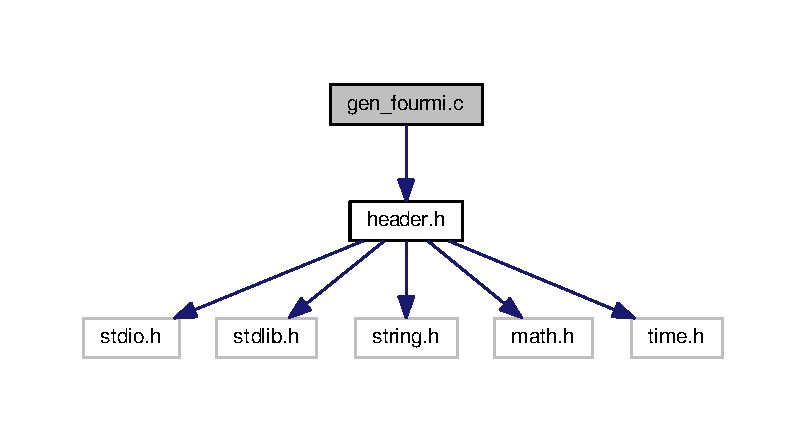
\includegraphics[width=350pt]{gen__fourmi_8c__incl}
\end{center}
\end{figure}
\subsection*{Fonctions}
\begin{DoxyCompactItemize}
\item 
void \hyperlink{gen__fourmi_8c_ae621d3f12ff30448e45c4e134d049b03}{gen\+\_\+fourmi} (void)
\begin{DoxyCompactList}\small\item\em Fonction permettant le pop des fourmis. \end{DoxyCompactList}\item 
void \hyperlink{gen__fourmi_8c_ae0cc7c685736b97de5cd92845f3730d3}{gen\+\_\+stock\+\_\+fourmi} (int id\+\_\+fourmi)
\begin{DoxyCompactList}\small\item\em Fonction permettant de definir une quantite de nourriture, d'eau, de dodo que possede Zozor. \end{DoxyCompactList}\item 
void \hyperlink{gen__fourmi_8c_add23d0755a1059dab2f4e326d1c8f2c5}{etat\+\_\+fourmi} (int id\+\_\+fourmi)
\begin{DoxyCompactList}\small\item\em Fonction permettant d'afficher l'etat de Zozor, sa quantite de repas, d'eau et de sommeil disponible. \end{DoxyCompactList}\end{DoxyCompactItemize}


\subsection{Description détaillée}
Page contenant les fonctions relatives a la de Zozor et de tout ce qui y touche. 

\begin{DoxyAuthor}{Auteur}
Jean-\/baptiste Dubois, Provost Valentin, Dezere Florian 
\end{DoxyAuthor}
\begin{DoxyVersion}{Version}
1.\+0 
\end{DoxyVersion}
\begin{DoxyDate}{Date}
6 Janvier 2014 
\end{DoxyDate}


\subsection{Documentation des fonctions}
\hypertarget{gen__fourmi_8c_add23d0755a1059dab2f4e326d1c8f2c5}{\index{gen\+\_\+fourmi.\+c@{gen\+\_\+fourmi.\+c}!etat\+\_\+fourmi@{etat\+\_\+fourmi}}
\index{etat\+\_\+fourmi@{etat\+\_\+fourmi}!gen\+\_\+fourmi.\+c@{gen\+\_\+fourmi.\+c}}
\subsubsection[{etat\+\_\+fourmi}]{\setlength{\rightskip}{0pt plus 5cm}void etat\+\_\+fourmi (
\begin{DoxyParamCaption}
\item[{int}]{id\+\_\+fourmi}
\end{DoxyParamCaption}
)}}\label{gen__fourmi_8c_add23d0755a1059dab2f4e326d1c8f2c5}


Fonction permettant d'afficher l'etat de Zozor, sa quantite de repas, d'eau et de sommeil disponible. 

fonction permettant d'afficher l'etat de Zozor, sa quantite de repas, d'eau et de sommeil disponible


\begin{DoxyParams}{Paramètres}
{\em int} & id\+\_\+fourmi est l'identifiant de Zozor \\
\hline
\end{DoxyParams}
\hypertarget{gen__fourmi_8c_ae621d3f12ff30448e45c4e134d049b03}{\index{gen\+\_\+fourmi.\+c@{gen\+\_\+fourmi.\+c}!gen\+\_\+fourmi@{gen\+\_\+fourmi}}
\index{gen\+\_\+fourmi@{gen\+\_\+fourmi}!gen\+\_\+fourmi.\+c@{gen\+\_\+fourmi.\+c}}
\subsubsection[{gen\+\_\+fourmi}]{\setlength{\rightskip}{0pt plus 5cm}void gen\+\_\+fourmi (
\begin{DoxyParamCaption}
\item[{void}]{}
\end{DoxyParamCaption}
)}}\label{gen__fourmi_8c_ae621d3f12ff30448e45c4e134d049b03}


Fonction permettant le pop des fourmis. 

fonction permettant le pop de Zozor \hypertarget{gen__fourmi_8c_ae0cc7c685736b97de5cd92845f3730d3}{\index{gen\+\_\+fourmi.\+c@{gen\+\_\+fourmi.\+c}!gen\+\_\+stock\+\_\+fourmi@{gen\+\_\+stock\+\_\+fourmi}}
\index{gen\+\_\+stock\+\_\+fourmi@{gen\+\_\+stock\+\_\+fourmi}!gen\+\_\+fourmi.\+c@{gen\+\_\+fourmi.\+c}}
\subsubsection[{gen\+\_\+stock\+\_\+fourmi}]{\setlength{\rightskip}{0pt plus 5cm}void gen\+\_\+stock\+\_\+fourmi (
\begin{DoxyParamCaption}
\item[{int}]{id\+\_\+fourmi}
\end{DoxyParamCaption}
)}}\label{gen__fourmi_8c_ae0cc7c685736b97de5cd92845f3730d3}


Fonction permettant de definir une quantite de nourriture, d'eau, de dodo que possede Zozor. 

Fonction permettant de definir une quantite de nourriture, d'eau, de dodo que poss�de Zozor.


\begin{DoxyParams}{Paramètres}
{\em int} & id\+\_\+fourmi est l'identifiant de Zozor \\
\hline
\end{DoxyParams}

\hypertarget{gen__labyrinthe_8c}{\section{Référence du fichier gen\+\_\+labyrinthe.\+c}
\label{gen__labyrinthe_8c}\index{gen\+\_\+labyrinthe.\+c@{gen\+\_\+labyrinthe.\+c}}
}


Page contenant les fonctions relatives a la creation du labyrinthe, et la mise en place des points strategiques.  


{\ttfamily \#include \char`\"{}header.\+h\char`\"{}}\\*
Graphe des dépendances par inclusion de gen\+\_\+labyrinthe.\+c\+:
\nopagebreak
\begin{figure}[H]
\begin{center}
\leavevmode
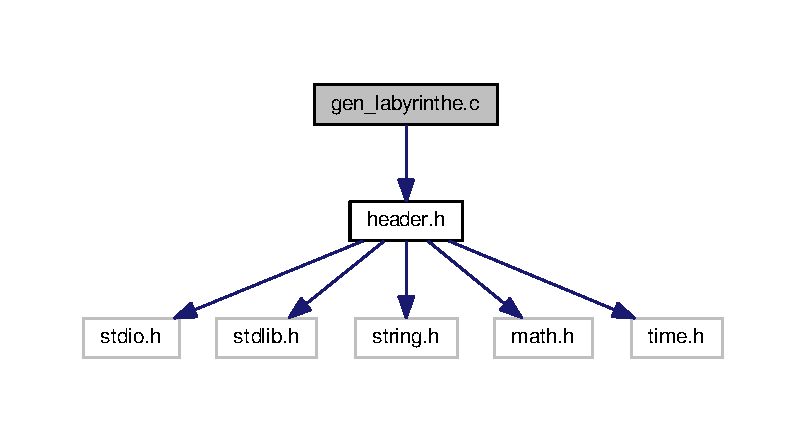
\includegraphics[width=350pt]{gen__labyrinthe_8c__incl}
\end{center}
\end{figure}
\subsection*{Fonctions}
\begin{DoxyCompactItemize}
\item 
\hypertarget{gen__labyrinthe_8c_a19f3e01f44b59e829cc792a8fd740228}{void \hyperlink{gen__labyrinthe_8c_a19f3e01f44b59e829cc792a8fd740228}{gen\+\_\+labyrinthe} (void)}\label{gen__labyrinthe_8c_a19f3e01f44b59e829cc792a8fd740228}

\begin{DoxyCompactList}\small\item\em Fonction de generation du labyrinthe. \end{DoxyCompactList}\item 
void \hyperlink{gen__labyrinthe_8c_afe6bbf858e6995f440df1523eef19bc8}{gen\+\_\+points\+\_\+eau} (int nb\+\_\+eau)
\begin{DoxyCompactList}\small\item\em Fonction de genration des differents points d'eau dans le labyrinthe. \end{DoxyCompactList}\item 
void \hyperlink{gen__labyrinthe_8c_a3dbb394bcc0a6496cfd3b905ab8b6c6c}{gen\+\_\+points\+\_\+repas} (int nb\+\_\+manger)
\begin{DoxyCompactList}\small\item\em Fonction de generation des differents points de manger dans le labyrinthe. \end{DoxyCompactList}\item 
\hypertarget{gen__labyrinthe_8c_adb09e0b6478d231ae9eb6898b6fc1686}{void {\bfseries gen\+\_\+points\+\_\+dodo} (int nb\+\_\+dodo)}\label{gen__labyrinthe_8c_adb09e0b6478d231ae9eb6898b6fc1686}

\item 
\hypertarget{gen__labyrinthe_8c_a72aad31dcd4e03575625ae0c64520761}{void {\bfseries gen\+\_\+points} (void)}\label{gen__labyrinthe_8c_a72aad31dcd4e03575625ae0c64520761}

\end{DoxyCompactItemize}


\subsection{Description détaillée}
Page contenant les fonctions relatives a la creation du labyrinthe, et la mise en place des points strategiques. 

\begin{DoxyAuthor}{Auteur}
Jean-\/baptiste Dubois, Provost Valentin, Dezere Florian 
\end{DoxyAuthor}
\begin{DoxyVersion}{Version}
1.\+0 
\end{DoxyVersion}
\begin{DoxyDate}{Date}
6 Janvier 2014 
\end{DoxyDate}


\subsection{Documentation des fonctions}
\hypertarget{gen__labyrinthe_8c_afe6bbf858e6995f440df1523eef19bc8}{\index{gen\+\_\+labyrinthe.\+c@{gen\+\_\+labyrinthe.\+c}!gen\+\_\+points\+\_\+eau@{gen\+\_\+points\+\_\+eau}}
\index{gen\+\_\+points\+\_\+eau@{gen\+\_\+points\+\_\+eau}!gen\+\_\+labyrinthe.\+c@{gen\+\_\+labyrinthe.\+c}}
\subsubsection[{gen\+\_\+points\+\_\+eau}]{\setlength{\rightskip}{0pt plus 5cm}void gen\+\_\+points\+\_\+eau (
\begin{DoxyParamCaption}
\item[{int}]{nb\+\_\+eau}
\end{DoxyParamCaption}
)}}\label{gen__labyrinthe_8c_afe6bbf858e6995f440df1523eef19bc8}


Fonction de genration des differents points d'eau dans le labyrinthe. 


\begin{DoxyParams}{Paramètres}
{\em int} & nb\+\_\+eau nombre de point d'eau a généré \\
\hline
\end{DoxyParams}
\hypertarget{gen__labyrinthe_8c_a3dbb394bcc0a6496cfd3b905ab8b6c6c}{\index{gen\+\_\+labyrinthe.\+c@{gen\+\_\+labyrinthe.\+c}!gen\+\_\+points\+\_\+repas@{gen\+\_\+points\+\_\+repas}}
\index{gen\+\_\+points\+\_\+repas@{gen\+\_\+points\+\_\+repas}!gen\+\_\+labyrinthe.\+c@{gen\+\_\+labyrinthe.\+c}}
\subsubsection[{gen\+\_\+points\+\_\+repas}]{\setlength{\rightskip}{0pt plus 5cm}void gen\+\_\+points\+\_\+repas (
\begin{DoxyParamCaption}
\item[{int}]{nb\+\_\+manger}
\end{DoxyParamCaption}
)}}\label{gen__labyrinthe_8c_a3dbb394bcc0a6496cfd3b905ab8b6c6c}


Fonction de generation des differents points de manger dans le labyrinthe. 


\begin{DoxyParams}{Paramètres}
{\em int} & nb\+\_\+manger nombre de point pour manger a généré \\
\hline
\end{DoxyParams}

\hypertarget{header_8h}{\section{Référence du fichier header.\+h}
\label{header_8h}\index{header.\+h@{header.\+h}}
}


Header contenant les definition des fonctions necessaire au \hyperlink{main_8c}{main.\+c}.  


{\ttfamily \#include $<$stdio.\+h$>$}\\*
{\ttfamily \#include $<$stdlib.\+h$>$}\\*
{\ttfamily \#include $<$string.\+h$>$}\\*
{\ttfamily \#include $<$math.\+h$>$}\\*
{\ttfamily \#include $<$time.\+h$>$}\\*
Graphe des dépendances par inclusion de header.\+h\+:
\nopagebreak
\begin{figure}[H]
\begin{center}
\leavevmode
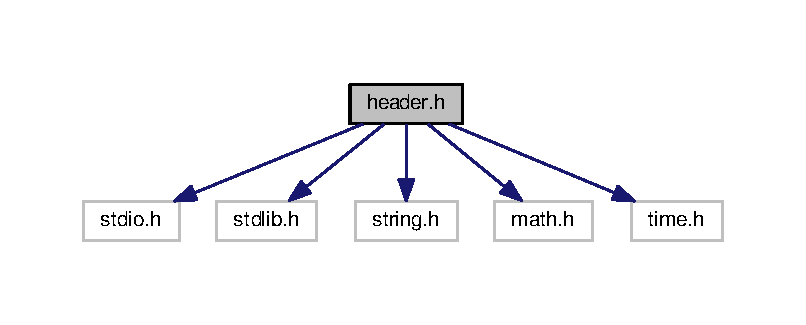
\includegraphics[width=350pt]{header_8h__incl}
\end{center}
\end{figure}
Ce graphe montre quels fichiers incluent directement ou indirectement ce fichier \+:
\nopagebreak
\begin{figure}[H]
\begin{center}
\leavevmode
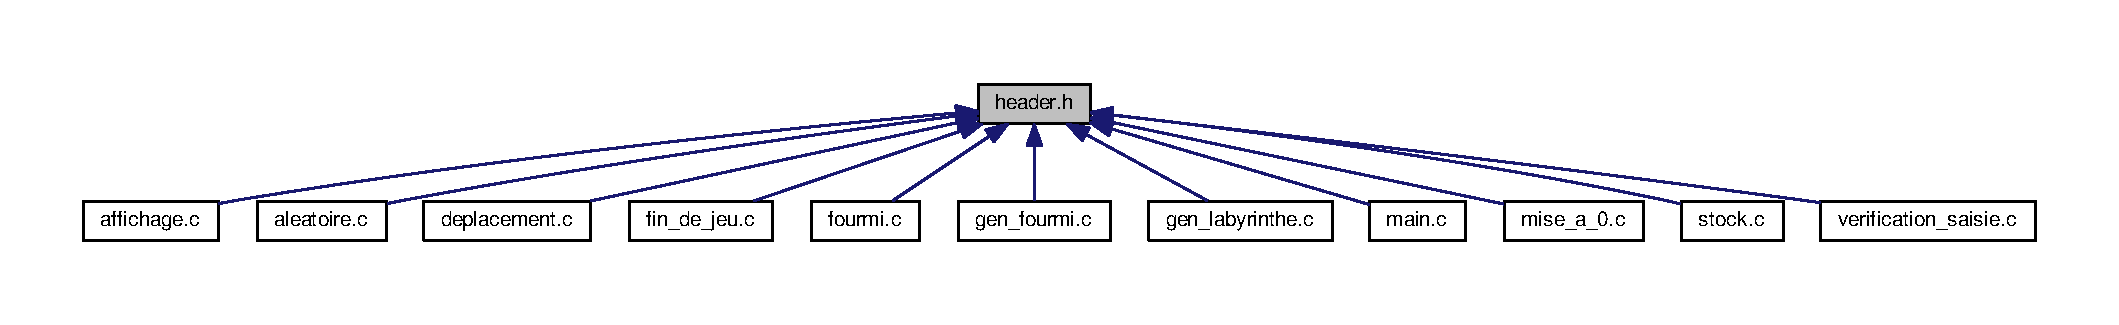
\includegraphics[width=350pt]{header_8h__dep__incl}
\end{center}
\end{figure}
\subsection*{Classes}
\begin{DoxyCompactItemize}
\item 
struct \hyperlink{structt__fourmi}{t\+\_\+fourmi}
\begin{DoxyCompactList}\small\item\em structure necessaire a la connaissance de Zozor, avec sa place en x, y et son numero d'immatriculation \end{DoxyCompactList}\end{DoxyCompactItemize}
\subsection*{Macros}
\begin{DoxyCompactItemize}
\item 
\hypertarget{header_8h_a0240ac851181b84ac374872dc5434ee4}{\#define {\bfseries N}~12}\label{header_8h_a0240ac851181b84ac374872dc5434ee4}

\item 
\hypertarget{header_8h_a51591cf51bdd6c1f6015532422e7770e}{\#define {\bfseries Z}~50}\label{header_8h_a51591cf51bdd6c1f6015532422e7770e}

\end{DoxyCompactItemize}
\subsection*{Énumérations}
\begin{DoxyCompactItemize}
\item 
\hypertarget{header_8h_ab21a60e1517c8d253cc83c12f6e027f3}{enum \hyperlink{header_8h_ab21a60e1517c8d253cc83c12f6e027f3}{t\+\_\+case} \{ \\*
{\bfseries vide}, 
{\bfseries mur}, 
{\bfseries base}, 
{\bfseries eau}, 
\\*
{\bfseries dodo}, 
{\bfseries manger}, 
{\bfseries fourmi}, 
{\bfseries troll\+\_\+case}
 \}}\label{header_8h_ab21a60e1517c8d253cc83c12f6e027f3}

\begin{DoxyCompactList}\small\item\em definition d'une énumération de type t\+\_\+case pour la création des differentes cases du labyrinthe \end{DoxyCompactList}\end{DoxyCompactItemize}
\subsection*{Fonctions}
\begin{DoxyCompactItemize}
\item 
\hypertarget{header_8h_a1c2fa03ead9cabe7107805a0388ed268}{void \hyperlink{header_8h_a1c2fa03ead9cabe7107805a0388ed268}{init\+\_\+labyrinthe} (void)}\label{header_8h_a1c2fa03ead9cabe7107805a0388ed268}

\begin{DoxyCompactList}\small\item\em Fonction d'initialisation de la matrice du labyrinthe a vide. \end{DoxyCompactList}\item 
\hypertarget{header_8h_a10e7f695f5aa9fec445332d9f45593f5}{void {\bfseries vide\+\_\+stock} (void)}\label{header_8h_a10e7f695f5aa9fec445332d9f45593f5}

\item 
\hypertarget{header_8h_a19f3e01f44b59e829cc792a8fd740228}{void \hyperlink{header_8h_a19f3e01f44b59e829cc792a8fd740228}{gen\+\_\+labyrinthe} (void)}\label{header_8h_a19f3e01f44b59e829cc792a8fd740228}

\begin{DoxyCompactList}\small\item\em Fonction de generation du labyrinthe. \end{DoxyCompactList}\item 
\hypertarget{header_8h_a42ec04270a0e1a044bcbec3d08bc9f0a}{void \hyperlink{header_8h_a42ec04270a0e1a044bcbec3d08bc9f0a}{affiche\+\_\+lab} (void)}\label{header_8h_a42ec04270a0e1a044bcbec3d08bc9f0a}

\begin{DoxyCompactList}\small\item\em Fonction d'affichage du labyrinthe. \end{DoxyCompactList}\item 
void \hyperlink{header_8h_afe6bbf858e6995f440df1523eef19bc8}{gen\+\_\+points\+\_\+eau} (int nb\+\_\+eau)
\begin{DoxyCompactList}\small\item\em Fonction de genration des differents points d'eau dans le labyrinthe. \end{DoxyCompactList}\item 
void \hyperlink{header_8h_ac944966f1f411455d5d9e1428e4d927d}{gen\+\_\+points\+\_\+repas} (int nb\+\_\+repas)
\begin{DoxyCompactList}\small\item\em Fonction de generation des differents points de manger dans le labyrinthe. \end{DoxyCompactList}\item 
void \hyperlink{header_8h_adb09e0b6478d231ae9eb6898b6fc1686}{gen\+\_\+points\+\_\+dodo} (int nb\+\_\+dodo)
\begin{DoxyCompactList}\small\item\em Fonction de generation des differents points de dodo dans le labyrinthe. \end{DoxyCompactList}\item 
\hypertarget{header_8h_a72aad31dcd4e03575625ae0c64520761}{void \hyperlink{header_8h_a72aad31dcd4e03575625ae0c64520761}{gen\+\_\+points} (void)}\label{header_8h_a72aad31dcd4e03575625ae0c64520761}

\begin{DoxyCompactList}\small\item\em Fonction de generation aleatoire des differents points utiles. \end{DoxyCompactList}\item 
\hypertarget{header_8h_ae2c76cb469b294db918d9f761ba445f9}{void {\bfseries gen\+\_\+stock} (void)}\label{header_8h_ae2c76cb469b294db918d9f761ba445f9}

\item 
void \hyperlink{header_8h_ae621d3f12ff30448e45c4e134d049b03}{gen\+\_\+fourmi} (void)
\begin{DoxyCompactList}\small\item\em Fonction permettant le pop des fourmis. \end{DoxyCompactList}\item 
void \hyperlink{header_8h_ae0cc7c685736b97de5cd92845f3730d3}{gen\+\_\+stock\+\_\+fourmi} (int id\+\_\+fourmi)
\begin{DoxyCompactList}\small\item\em Fonction permettant de definir une quantite de nourriture, d'eau, de dodo que possede Zozor. \end{DoxyCompactList}\item 
void \hyperlink{header_8h_a851f3d658198e4622f03e2d8a7faec14}{mv\+\_\+fourmi} (int id\+\_\+fourmi)
\begin{DoxyCompactList}\small\item\em Fonction permettant le deplacement des fourmis dans le labyrinthe de fa�on aleatoire. \end{DoxyCompactList}\item 
\hypertarget{header_8h_a5b977cd2b36e961cb4b9382e91ade34b}{int \hyperlink{header_8h_a5b977cd2b36e961cb4b9382e91ade34b}{end\+\_\+game} (void)}\label{header_8h_a5b977cd2b36e961cb4b9382e91ade34b}

\begin{DoxyCompactList}\small\item\em Fonction permettant de savoir si la troll case met fin a la partie. \end{DoxyCompactList}\item 
int \hyperlink{header_8h_a022b37db62e51a6efc03eee80cda50cd}{verif\+\_\+deplacement} (int id\+\_\+fourmi)
\begin{DoxyCompactList}\small\item\em Fonction permettant de verifier si Zozor peut se deplacer. \end{DoxyCompactList}\item 
void \hyperlink{header_8h_add23d0755a1059dab2f4e326d1c8f2c5}{etat\+\_\+fourmi} (int id\+\_\+fourmi)
\begin{DoxyCompactList}\small\item\em Fonction permettant d'afficher l'etat de Zozor, sa quantite de repas, d'eau et de sommeil disponible. \end{DoxyCompactList}\item 
\hypertarget{header_8h_ad9fd7e15b3676ff1d6f05821968adf54}{void \hyperlink{header_8h_ad9fd7e15b3676ff1d6f05821968adf54}{gen\+\_\+troll\+\_\+case} (void)}\label{header_8h_ad9fd7e15b3676ff1d6f05821968adf54}

\begin{DoxyCompactList}\small\item\em Fonction permettant la generation de la troll case, qui peut mettre fin a la partie. \end{DoxyCompactList}\item 
void \hyperlink{header_8h_a85661a77431adbf32f45d1b707c270e2}{recherche\+\_\+base} (int $\ast$x, int $\ast$y)
\begin{DoxyCompactList}\small\item\em Fonction permettant la recherche de la base du labyrinthe pour le pop de Zozor. \end{DoxyCompactList}\item 
int \hyperlink{header_8h_a5d77334ef0eb544c90e47f78b6e898cd}{verif\+\_\+saisie} (int petit, int grand)
\begin{DoxyCompactList}\small\item\em Fonction permettant de verifier si la saisie de l'utilisateur est correcte. \end{DoxyCompactList}\item 
void \hyperlink{header_8h_afdabedbdaec06f1a4ab234044b4df6fc}{affiche\+\_\+entrer} (int tmp)
\begin{DoxyCompactList}\small\item\em Fonction permettant l'affichage d'un certain nombre de ligne vide. \end{DoxyCompactList}\item 
\hypertarget{header_8h_aaeeedbd134251291fe79c71c943ec899}{void \hyperlink{header_8h_aaeeedbd134251291fe79c71c943ec899}{aleatoire} (void)}\label{header_8h_aaeeedbd134251291fe79c71c943ec899}

\begin{DoxyCompactList}\small\item\em Fonction permettant de creer l'aleatoire. \end{DoxyCompactList}\end{DoxyCompactItemize}
\subsection*{Variables}
\begin{DoxyCompactItemize}
\item 
\hypertarget{header_8h_ae63cd84fc42fbad761b2ec07b238d9f3}{\hyperlink{structt__fourmi}{t\+\_\+fourmi} {\bfseries population} \mbox{[}Z\mbox{]}}\label{header_8h_ae63cd84fc42fbad761b2ec07b238d9f3}

\item 
\hypertarget{header_8h_a2143372ed5e7e6c3e275568a5a62f085}{\hyperlink{header_8h_ab21a60e1517c8d253cc83c12f6e027f3}{t\+\_\+case} {\bfseries labyrinthe} \mbox{[}N\mbox{]}\mbox{[}N\mbox{]}}\label{header_8h_a2143372ed5e7e6c3e275568a5a62f085}

\item 
\hypertarget{header_8h_a3bd8eb4406b8694c8f4ce3496e52ea2d}{\hyperlink{header_8h_ab21a60e1517c8d253cc83c12f6e027f3}{t\+\_\+case} {\bfseries emplacement} \mbox{[}N\mbox{]}\mbox{[}N\mbox{]}}\label{header_8h_a3bd8eb4406b8694c8f4ce3496e52ea2d}

\item 
\hypertarget{header_8h_a6a30c7798b4d072c13948aeca1de524e}{int {\bfseries stock} \mbox{[}N\mbox{]}\mbox{[}N\mbox{]}}\label{header_8h_a6a30c7798b4d072c13948aeca1de524e}

\end{DoxyCompactItemize}


\subsection{Description détaillée}
Header contenant les definition des fonctions necessaire au \hyperlink{main_8c}{main.\+c}. 

\begin{DoxyAuthor}{Auteur}
Jean-\/baptiste Dubois, Provost Valentin, Dezere Florian 
\end{DoxyAuthor}
\begin{DoxyVersion}{Version}
1.\+0 
\end{DoxyVersion}
\begin{DoxyDate}{Date}
6 Janvier 2014 
\end{DoxyDate}


\subsection{Documentation des fonctions}
\hypertarget{header_8h_afdabedbdaec06f1a4ab234044b4df6fc}{\index{header.\+h@{header.\+h}!affiche\+\_\+entrer@{affiche\+\_\+entrer}}
\index{affiche\+\_\+entrer@{affiche\+\_\+entrer}!header.\+h@{header.\+h}}
\subsubsection[{affiche\+\_\+entrer}]{\setlength{\rightskip}{0pt plus 5cm}void affiche\+\_\+entrer (
\begin{DoxyParamCaption}
\item[{int}]{tmp}
\end{DoxyParamCaption}
)}}\label{header_8h_afdabedbdaec06f1a4ab234044b4df6fc}


Fonction permettant l'affichage d'un certain nombre de ligne vide. 


\begin{DoxyParams}{Paramètres}
{\em int} & tmp nombre de retour chariot � afficher \\
\hline
\end{DoxyParams}
\hypertarget{header_8h_add23d0755a1059dab2f4e326d1c8f2c5}{\index{header.\+h@{header.\+h}!etat\+\_\+fourmi@{etat\+\_\+fourmi}}
\index{etat\+\_\+fourmi@{etat\+\_\+fourmi}!header.\+h@{header.\+h}}
\subsubsection[{etat\+\_\+fourmi}]{\setlength{\rightskip}{0pt plus 5cm}void etat\+\_\+fourmi (
\begin{DoxyParamCaption}
\item[{int}]{id\+\_\+fourmi}
\end{DoxyParamCaption}
)}}\label{header_8h_add23d0755a1059dab2f4e326d1c8f2c5}


Fonction permettant d'afficher l'etat de Zozor, sa quantite de repas, d'eau et de sommeil disponible. 

fonction permettant d'afficher l'etat de Zozor, sa quantite de repas, d'eau et de sommeil disponible


\begin{DoxyParams}{Paramètres}
{\em int} & id\+\_\+fourmi est l'identifiant de Zozor \\
\hline
\end{DoxyParams}
\hypertarget{header_8h_ae621d3f12ff30448e45c4e134d049b03}{\index{header.\+h@{header.\+h}!gen\+\_\+fourmi@{gen\+\_\+fourmi}}
\index{gen\+\_\+fourmi@{gen\+\_\+fourmi}!header.\+h@{header.\+h}}
\subsubsection[{gen\+\_\+fourmi}]{\setlength{\rightskip}{0pt plus 5cm}void gen\+\_\+fourmi (
\begin{DoxyParamCaption}
\item[{void}]{}
\end{DoxyParamCaption}
)}}\label{header_8h_ae621d3f12ff30448e45c4e134d049b03}


Fonction permettant le pop des fourmis. 

fonction permettant le pop de Zozor \hypertarget{header_8h_adb09e0b6478d231ae9eb6898b6fc1686}{\index{header.\+h@{header.\+h}!gen\+\_\+points\+\_\+dodo@{gen\+\_\+points\+\_\+dodo}}
\index{gen\+\_\+points\+\_\+dodo@{gen\+\_\+points\+\_\+dodo}!header.\+h@{header.\+h}}
\subsubsection[{gen\+\_\+points\+\_\+dodo}]{\setlength{\rightskip}{0pt plus 5cm}void gen\+\_\+points\+\_\+dodo (
\begin{DoxyParamCaption}
\item[{int}]{nb\+\_\+dodo}
\end{DoxyParamCaption}
)}}\label{header_8h_adb09e0b6478d231ae9eb6898b6fc1686}


Fonction de generation des differents points de dodo dans le labyrinthe. 


\begin{DoxyParams}{Paramètres}
{\em int} & nb\+\_\+dodo nombre de point pour dormir a généré \\
\hline
\end{DoxyParams}
\hypertarget{header_8h_afe6bbf858e6995f440df1523eef19bc8}{\index{header.\+h@{header.\+h}!gen\+\_\+points\+\_\+eau@{gen\+\_\+points\+\_\+eau}}
\index{gen\+\_\+points\+\_\+eau@{gen\+\_\+points\+\_\+eau}!header.\+h@{header.\+h}}
\subsubsection[{gen\+\_\+points\+\_\+eau}]{\setlength{\rightskip}{0pt plus 5cm}void gen\+\_\+points\+\_\+eau (
\begin{DoxyParamCaption}
\item[{int}]{nb\+\_\+eau}
\end{DoxyParamCaption}
)}}\label{header_8h_afe6bbf858e6995f440df1523eef19bc8}


Fonction de genration des differents points d'eau dans le labyrinthe. 


\begin{DoxyParams}{Paramètres}
{\em int} & nb\+\_\+eau nombre de point d'eau a généré \\
\hline
\end{DoxyParams}
\hypertarget{header_8h_ac944966f1f411455d5d9e1428e4d927d}{\index{header.\+h@{header.\+h}!gen\+\_\+points\+\_\+repas@{gen\+\_\+points\+\_\+repas}}
\index{gen\+\_\+points\+\_\+repas@{gen\+\_\+points\+\_\+repas}!header.\+h@{header.\+h}}
\subsubsection[{gen\+\_\+points\+\_\+repas}]{\setlength{\rightskip}{0pt plus 5cm}void gen\+\_\+points\+\_\+repas (
\begin{DoxyParamCaption}
\item[{int}]{nb\+\_\+manger}
\end{DoxyParamCaption}
)}}\label{header_8h_ac944966f1f411455d5d9e1428e4d927d}


Fonction de generation des differents points de manger dans le labyrinthe. 


\begin{DoxyParams}{Paramètres}
{\em int} & nb\+\_\+manger nombre de point pour manger a généré \\
\hline
\end{DoxyParams}
\hypertarget{header_8h_ae0cc7c685736b97de5cd92845f3730d3}{\index{header.\+h@{header.\+h}!gen\+\_\+stock\+\_\+fourmi@{gen\+\_\+stock\+\_\+fourmi}}
\index{gen\+\_\+stock\+\_\+fourmi@{gen\+\_\+stock\+\_\+fourmi}!header.\+h@{header.\+h}}
\subsubsection[{gen\+\_\+stock\+\_\+fourmi}]{\setlength{\rightskip}{0pt plus 5cm}void gen\+\_\+stock\+\_\+fourmi (
\begin{DoxyParamCaption}
\item[{int}]{id\+\_\+fourmi}
\end{DoxyParamCaption}
)}}\label{header_8h_ae0cc7c685736b97de5cd92845f3730d3}


Fonction permettant de definir une quantite de nourriture, d'eau, de dodo que possede Zozor. 

Fonction permettant de definir une quantite de nourriture, d'eau, de dodo que poss�de Zozor.


\begin{DoxyParams}{Paramètres}
{\em int} & id\+\_\+fourmi est l'identifiant de Zozor \\
\hline
\end{DoxyParams}
\hypertarget{header_8h_a851f3d658198e4622f03e2d8a7faec14}{\index{header.\+h@{header.\+h}!mv\+\_\+fourmi@{mv\+\_\+fourmi}}
\index{mv\+\_\+fourmi@{mv\+\_\+fourmi}!header.\+h@{header.\+h}}
\subsubsection[{mv\+\_\+fourmi}]{\setlength{\rightskip}{0pt plus 5cm}void mv\+\_\+fourmi (
\begin{DoxyParamCaption}
\item[{int}]{id\+\_\+fourmi}
\end{DoxyParamCaption}
)}}\label{header_8h_a851f3d658198e4622f03e2d8a7faec14}


Fonction permettant le deplacement des fourmis dans le labyrinthe de fa�on aleatoire. 


\begin{DoxyParams}{Paramètres}
{\em int} & id\+\_\+fourmi est l'identifiant de Zozor \\
\hline
\end{DoxyParams}
\hypertarget{header_8h_a85661a77431adbf32f45d1b707c270e2}{\index{header.\+h@{header.\+h}!recherche\+\_\+base@{recherche\+\_\+base}}
\index{recherche\+\_\+base@{recherche\+\_\+base}!header.\+h@{header.\+h}}
\subsubsection[{recherche\+\_\+base}]{\setlength{\rightskip}{0pt plus 5cm}void recherche\+\_\+base (
\begin{DoxyParamCaption}
\item[{int $\ast$}]{x, }
\item[{int $\ast$}]{y}
\end{DoxyParamCaption}
)}}\label{header_8h_a85661a77431adbf32f45d1b707c270e2}


Fonction permettant la recherche de la base du labyrinthe pour le pop de Zozor. 


\begin{DoxyParams}{Paramètres}
{\em int} & $\ast$x, int $\ast$y sont des pointeurs qui permettent de r�cuperer les valeurs pour la base \\
\hline
\end{DoxyParams}
\hypertarget{header_8h_a022b37db62e51a6efc03eee80cda50cd}{\index{header.\+h@{header.\+h}!verif\+\_\+deplacement@{verif\+\_\+deplacement}}
\index{verif\+\_\+deplacement@{verif\+\_\+deplacement}!header.\+h@{header.\+h}}
\subsubsection[{verif\+\_\+deplacement}]{\setlength{\rightskip}{0pt plus 5cm}int verif\+\_\+deplacement (
\begin{DoxyParamCaption}
\item[{int}]{id\+\_\+fourmi}
\end{DoxyParamCaption}
)}}\label{header_8h_a022b37db62e51a6efc03eee80cda50cd}


Fonction permettant de verifier si Zozor peut se deplacer. 


\begin{DoxyParams}{Paramètres}
{\em int} & id\+\_\+fourmi est l'identifiant de Zozor \\
\hline
\end{DoxyParams}
\begin{DoxyReturn}{Renvoie}
renvoi vrai si le d�placement peut avoir lieu sinon faux 
\end{DoxyReturn}
\hypertarget{header_8h_a5d77334ef0eb544c90e47f78b6e898cd}{\index{header.\+h@{header.\+h}!verif\+\_\+saisie@{verif\+\_\+saisie}}
\index{verif\+\_\+saisie@{verif\+\_\+saisie}!header.\+h@{header.\+h}}
\subsubsection[{verif\+\_\+saisie}]{\setlength{\rightskip}{0pt plus 5cm}int verif\+\_\+saisie (
\begin{DoxyParamCaption}
\item[{int}]{petit, }
\item[{int}]{grand}
\end{DoxyParamCaption}
)}}\label{header_8h_a5d77334ef0eb544c90e47f78b6e898cd}


Fonction permettant de verifier si la saisie de l'utilisateur est correcte. 


\begin{DoxyParams}{Paramètres}
{\em int} & petit, int grand param�tre pour verifier si le nombre entrer n'est pas trop grand ou trop petit \\
\hline
\end{DoxyParams}
\begin{DoxyReturn}{Renvoie}
renvoi le nombre entrer par l'utilisateur 
\end{DoxyReturn}

\hypertarget{header__fourmi_8h}{\section{Référence du fichier header\+\_\+fourmi.\+h}
\label{header__fourmi_8h}\index{header\+\_\+fourmi.\+h@{header\+\_\+fourmi.\+h}}
}


Header contenant les definition des fonctions necessaire au fonction de génération des fourmis et de leurs déplacements.  


Ce graphe montre quels fichiers incluent directement ou indirectement ce fichier \+:
\nopagebreak
\begin{figure}[H]
\begin{center}
\leavevmode
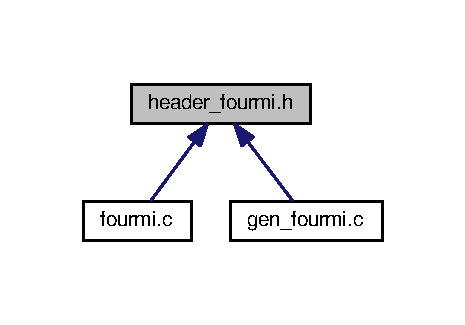
\includegraphics[width=223pt]{header__fourmi_8h__dep__incl}
\end{center}
\end{figure}
\subsection*{Variables}
\begin{DoxyCompactItemize}
\item 
\hypertarget{header__fourmi_8h_a3af0be4bdbdb4be8fd3af7360873650d}{int {\bfseries nb\+\_\+fourmi} = 0}\label{header__fourmi_8h_a3af0be4bdbdb4be8fd3af7360873650d}

\end{DoxyCompactItemize}


\subsection{Description détaillée}
Header contenant les definition des fonctions necessaire au fonction de génération des fourmis et de leurs déplacements. 

\begin{DoxyAuthor}{Auteur}
Jean-\/baptiste Dubois, Provost Valentin, Dezere Florian 
\end{DoxyAuthor}
\begin{DoxyVersion}{Version}
1.\+0 
\end{DoxyVersion}
\begin{DoxyDate}{Date}
6 Janvier 2014 
\end{DoxyDate}

\hypertarget{main_8c}{\section{Référence du fichier main.\+c}
\label{main_8c}\index{main.\+c@{main.\+c}}
}


Simulation de la vie d'un groupe de Zozor dans un labyrinthe.  


{\ttfamily \#include \char`\"{}header.\+h\char`\"{}}\\*
Graphe des dépendances par inclusion de main.\+c\+:
\nopagebreak
\begin{figure}[H]
\begin{center}
\leavevmode
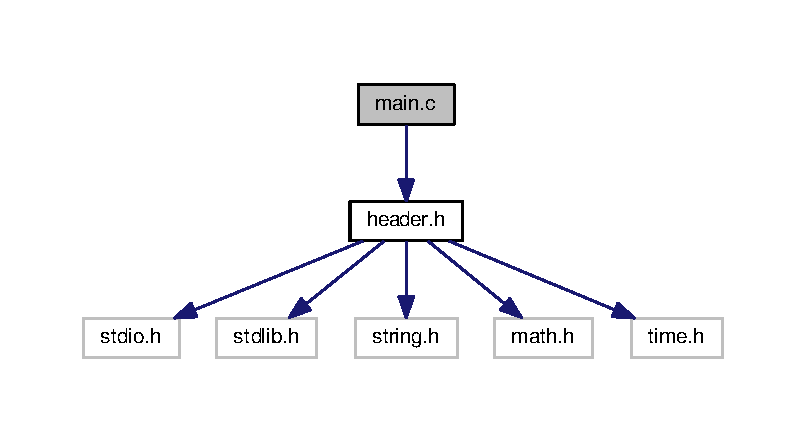
\includegraphics[width=350pt]{main_8c__incl}
\end{center}
\end{figure}
\subsection*{Fonctions}
\begin{DoxyCompactItemize}
\item 
\hypertarget{main_8c_a840291bc02cba5474a4cb46a9b9566fe}{int {\bfseries main} (void)}\label{main_8c_a840291bc02cba5474a4cb46a9b9566fe}

\end{DoxyCompactItemize}


\subsection{Description détaillée}
Simulation de la vie d'un groupe de Zozor dans un labyrinthe. 

\begin{DoxyAuthor}{Auteur}
Jean-\/baptiste Dubois, Provost Valentin, Dezere Florian 
\end{DoxyAuthor}
\begin{DoxyVersion}{Version}
1.\+0 
\end{DoxyVersion}
\begin{DoxyDate}{Date}
6 Janvier 2014 
\end{DoxyDate}

\hypertarget{mise__a__0_8c}{\section{Référence du fichier mise\+\_\+a\+\_\+0.\+c}
\label{mise__a__0_8c}\index{mise\+\_\+a\+\_\+0.\+c@{mise\+\_\+a\+\_\+0.\+c}}
}


D�finition des fonctions de mise a zero d'une matrice, ou de mise a l'�tat vide.  


{\ttfamily \#include \char`\"{}header.\+h\char`\"{}}\\*
Graphe des dépendances par inclusion de mise\+\_\+a\+\_\+0.\+c\+:
\nopagebreak
\begin{figure}[H]
\begin{center}
\leavevmode
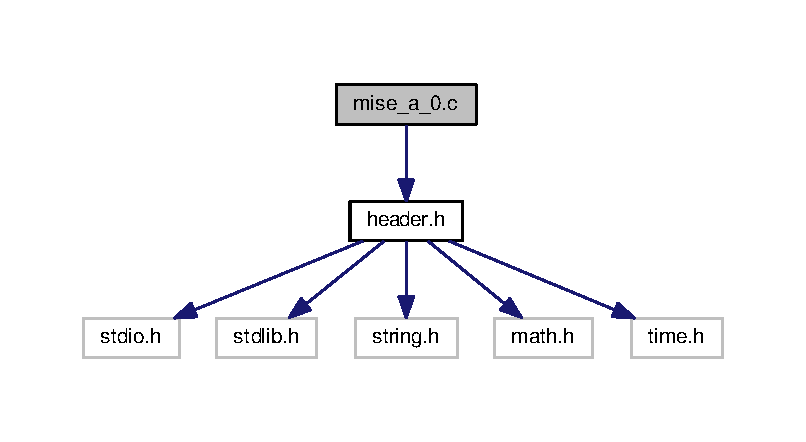
\includegraphics[width=350pt]{mise__a__0_8c__incl}
\end{center}
\end{figure}
\subsection*{Fonctions}
\begin{DoxyCompactItemize}
\item 
\hypertarget{mise__a__0_8c_a1c2fa03ead9cabe7107805a0388ed268}{void \hyperlink{mise__a__0_8c_a1c2fa03ead9cabe7107805a0388ed268}{init\+\_\+labyrinthe} (void)}\label{mise__a__0_8c_a1c2fa03ead9cabe7107805a0388ed268}

\begin{DoxyCompactList}\small\item\em Fonction d'initialisation de la matrice du labyrinthe a vide. \end{DoxyCompactList}\item 
\hypertarget{mise__a__0_8c_a10e7f695f5aa9fec445332d9f45593f5}{void {\bfseries vide\+\_\+stock} (void)}\label{mise__a__0_8c_a10e7f695f5aa9fec445332d9f45593f5}

\end{DoxyCompactItemize}


\subsection{Description détaillée}
D�finition des fonctions de mise a zero d'une matrice, ou de mise a l'�tat vide. 

\begin{DoxyAuthor}{Auteur}
Jean-\/baptiste Dubois, Provost Valentin, Dezere Florian 
\end{DoxyAuthor}
\begin{DoxyVersion}{Version}
1.\+0 
\end{DoxyVersion}
\begin{DoxyDate}{Date}
6 Janvier 2014 
\end{DoxyDate}

\hypertarget{stock_8c}{\section{Référence du fichier stock.\+c}
\label{stock_8c}\index{stock.\+c@{stock.\+c}}
}


D�finition des fonctions permettant de gerer les stocks de chaques points, de la cr�ation au retrait.  


{\ttfamily \#include \char`\"{}header.\+h\char`\"{}}\\*
Graphe des dépendances par inclusion de stock.\+c\+:\nopagebreak
\begin{figure}[H]
\begin{center}
\leavevmode
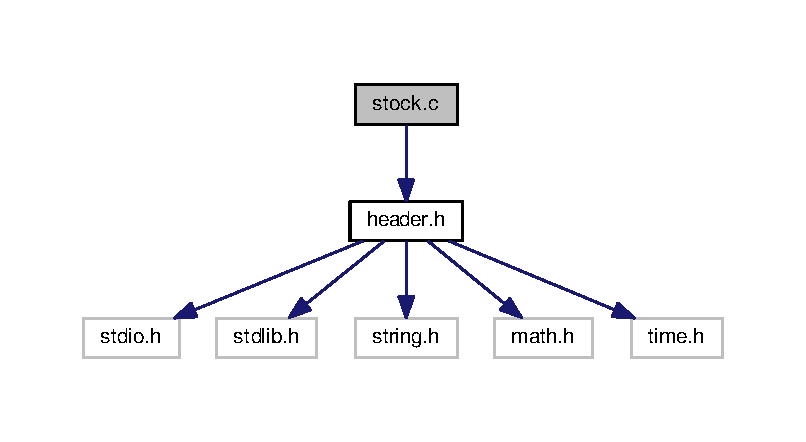
\includegraphics[width=350pt]{stock_8c__incl}
\end{center}
\end{figure}
\subsection*{Fonctions}
\begin{DoxyCompactItemize}
\item 
\hypertarget{stock_8c_ae2c76cb469b294db918d9f761ba445f9}{void \hyperlink{stock_8c_ae2c76cb469b294db918d9f761ba445f9}{gen\+\_\+stock} (void)}\label{stock_8c_ae2c76cb469b294db918d9f761ba445f9}

\begin{DoxyCompactList}\small\item\em Fonction permettant de definir une quantite al�atoire de repas, d'eau ou de sommeil sur chaque point correspondant. \end{DoxyCompactList}\end{DoxyCompactItemize}


\subsection{Description détaillée}
D�finition des fonctions permettant de gerer les stocks de chaques points, de la cr�ation au retrait. 

\begin{DoxyAuthor}{Auteur}
Jean-\/baptiste Dubois, Provost Valentin, Dezere Florian 
\end{DoxyAuthor}
\begin{DoxyVersion}{Version}
1.\+0 
\end{DoxyVersion}
\begin{DoxyDate}{Date}
6 Janvier 2014 
\end{DoxyDate}

\hypertarget{verification__saisie_8c}{\section{Référence du fichier verification\+\_\+saisie.\+c}
\label{verification__saisie_8c}\index{verification\+\_\+saisie.\+c@{verification\+\_\+saisie.\+c}}
}


Page permettant de v�rifier la saisie de l'utilisateur.  


{\ttfamily \#include \char`\"{}header.\+h\char`\"{}}\\*
Graphe des dépendances par inclusion de verification\+\_\+saisie.\+c\+:\nopagebreak
\begin{figure}[H]
\begin{center}
\leavevmode
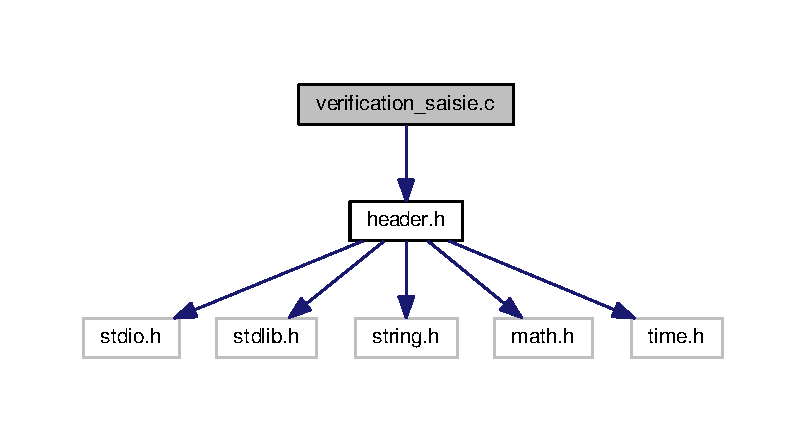
\includegraphics[width=350pt]{verification__saisie_8c__incl}
\end{center}
\end{figure}
\subsection*{Fonctions}
\begin{DoxyCompactItemize}
\item 
int \hyperlink{verification__saisie_8c_a5d77334ef0eb544c90e47f78b6e898cd}{verif\+\_\+saisie} (int petit, int grand)
\begin{DoxyCompactList}\small\item\em Fonction permettant de verifier si la saisie de l'utilisateur est correcte. \end{DoxyCompactList}\end{DoxyCompactItemize}


\subsection{Description détaillée}
Page permettant de v�rifier la saisie de l'utilisateur. 

\begin{DoxyAuthor}{Auteur}
Jean-\/baptiste Dubois, Provost Valentin, Dezere Florian 
\end{DoxyAuthor}
\begin{DoxyVersion}{Version}
1.\+0 
\end{DoxyVersion}
\begin{DoxyDate}{Date}
6 Janvier 2014 
\end{DoxyDate}


\subsection{Documentation des fonctions}
\hypertarget{verification__saisie_8c_a5d77334ef0eb544c90e47f78b6e898cd}{\index{verification\+\_\+saisie.\+c@{verification\+\_\+saisie.\+c}!verif\+\_\+saisie@{verif\+\_\+saisie}}
\index{verif\+\_\+saisie@{verif\+\_\+saisie}!verification\+\_\+saisie.\+c@{verification\+\_\+saisie.\+c}}
\subsubsection[{verif\+\_\+saisie}]{\setlength{\rightskip}{0pt plus 5cm}int verif\+\_\+saisie (
\begin{DoxyParamCaption}
\item[{int}]{petit, }
\item[{int}]{grand}
\end{DoxyParamCaption}
)}}\label{verification__saisie_8c_a5d77334ef0eb544c90e47f78b6e898cd}


Fonction permettant de verifier si la saisie de l'utilisateur est correcte. 


\begin{DoxyParams}{Paramètres}
{\em int} & petit, int grand param�tre pour verifier si le nombre entrer n'est pas trop grand ou trop petit \\
\hline
\end{DoxyParams}
\begin{DoxyReturn}{Renvoie}
renvoi le nombre entrer par l'utilisateur 
\end{DoxyReturn}

%--- End generated contents ---

% Index
\newpage
\phantomsection
\addcontentsline{toc}{chapter}{Index}
\printindex

\end{document}
